\documentclass[12pt]{article}
\usepackage{graphicx} % Required for inserting images
\usepackage{amsmath}
\usepackage{geometry}
\geometry{margin=1in}
\usepackage{amssymb}

\title{Population Econ HW2}
\author{YU HSIANG LIEN 1A202G34}
\date{November 2023}

\begin{document}

\maketitle

\section{Chapter 4}
\begin{enumerate}
    \item [\textbf{Q1}]
    $E_D = 1200 - 30w$, $E_S = 750$

    1. Since the labor supply is perfectly in-elastically, the number of workers\\ employed = 750

    2. To find the market wage $\Rightarrow 1200 - 30w = 750 \Rightarrow 30w = 450 \Rightarrow w = 15$

    3. Producer Surplus = $\frac{(40-15)750}{2} = 9375$

    \textbf{Ans}: Employed Workers = 750, Wage = 15, Producer Surplus = 9375
    
    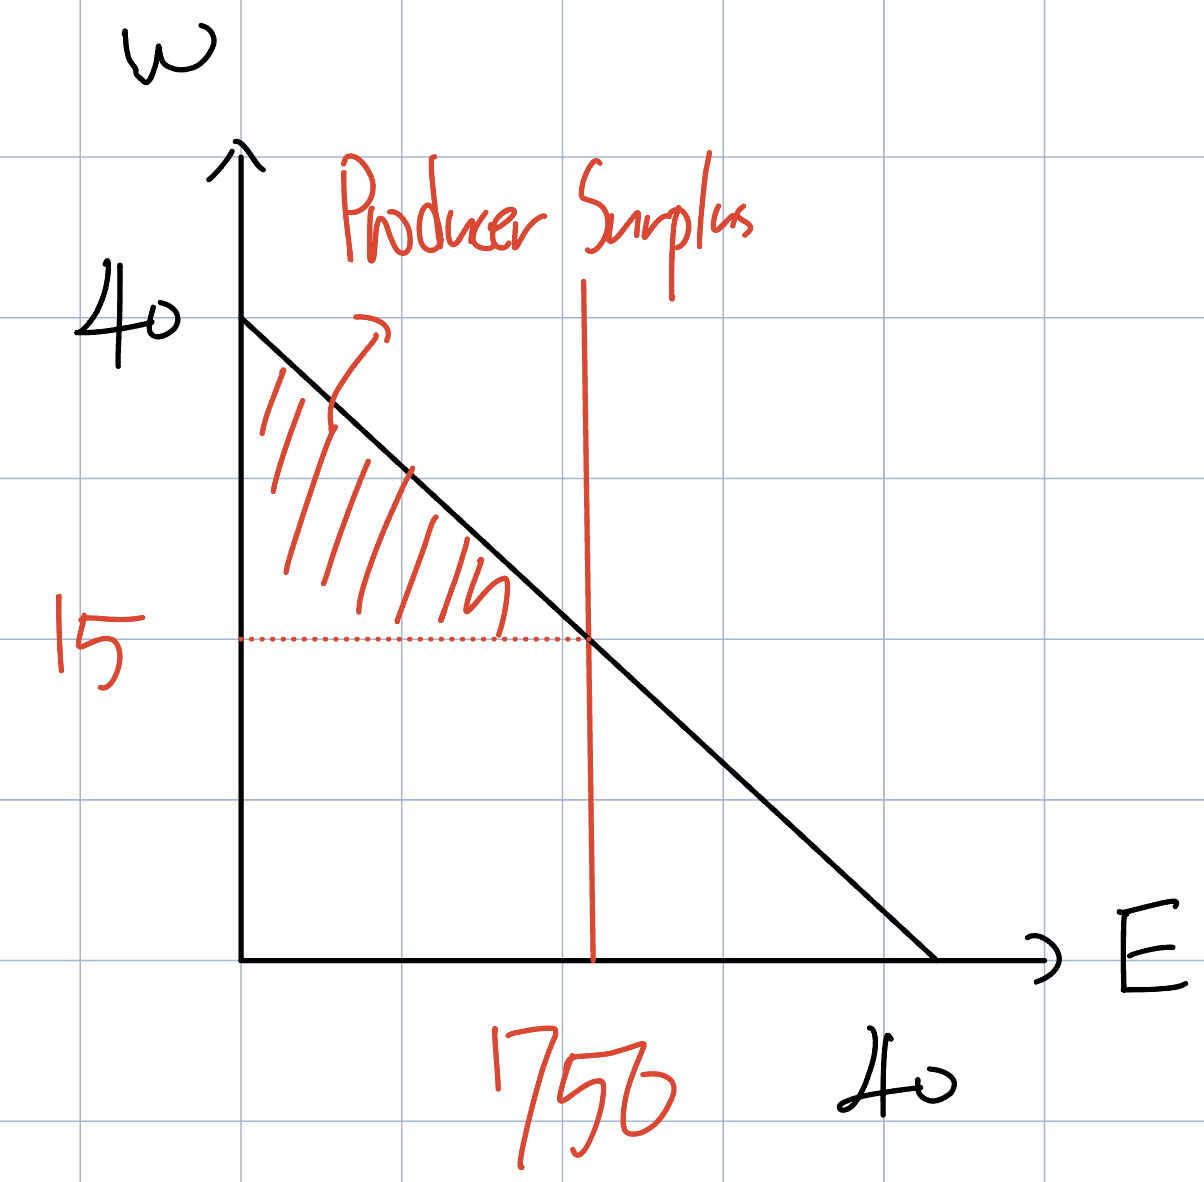
\includegraphics[width=0.5\linewidth]{IMG_0055C2D074BF-1.jpeg}

    \newpage
    \item [\textbf{Q2}]
    $E_D = 1000 - 50w$

    (a) When $E_S = 100w - 800$

    $\Rightarrow Market Equilibrium \Rightarrow 1000 - 50w = 100w - 800 \Rightarrow 1800 = 150w \Rightarrow \\w = 12$

    $E = 1000 - 600 = 400$

    Producer Surplus = $\frac{(20 - 12)400}{2} = 1600$

    \textbf{Ans}: Wage = 12, Employed Worker = 400, Producer Surplus = 1600

    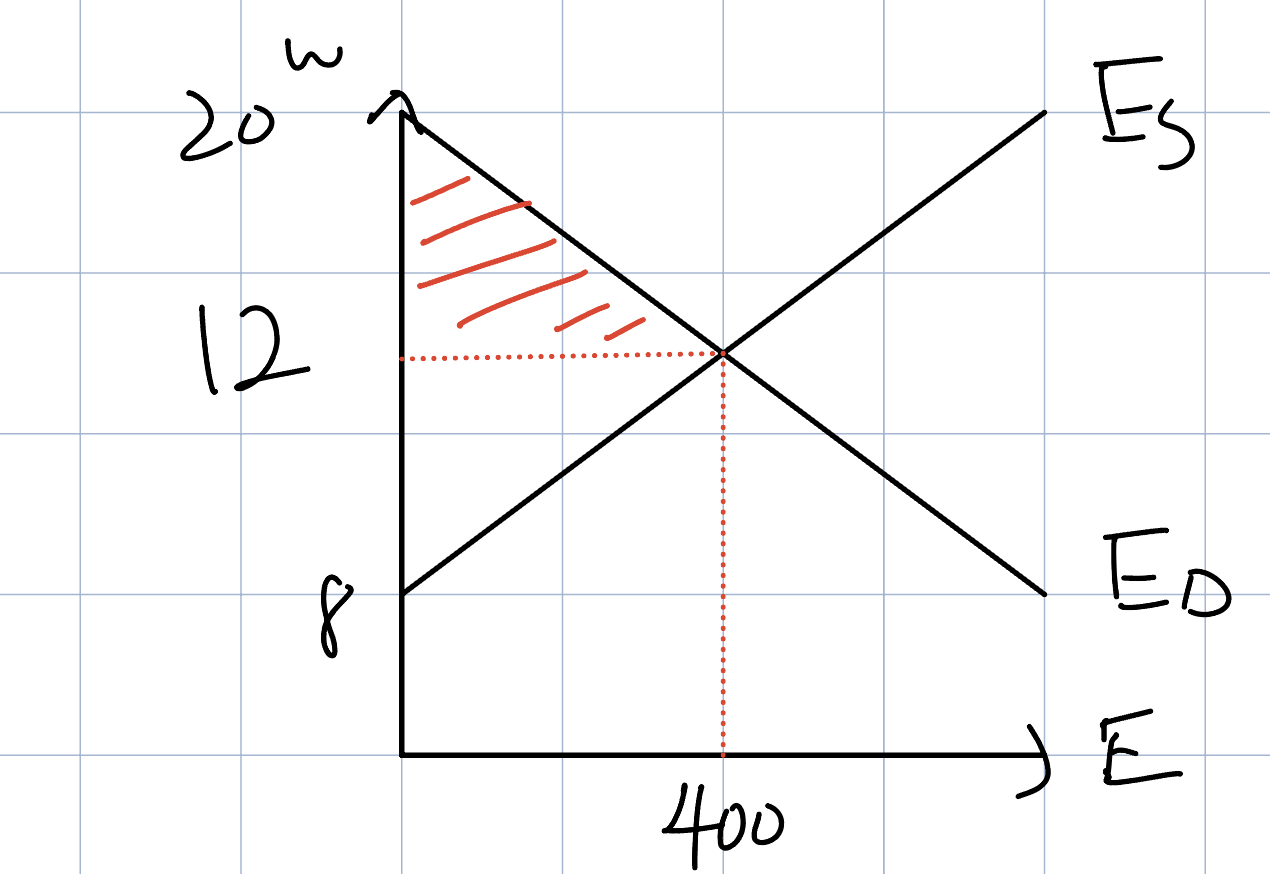
\includegraphics[width=0.5\linewidth]{IMG_CB85DBDA7A8E-1.jpeg}

    (b) Impose minimum wage of 16

    $E = 1000 - (50 \times 16) = 200$
    Producer Surplus = $\frac{(20-16)200}{2} = 400$

    \textbf{Ans}: Wage = 16, Employed Worker = 200, Producer Surplus = 400

    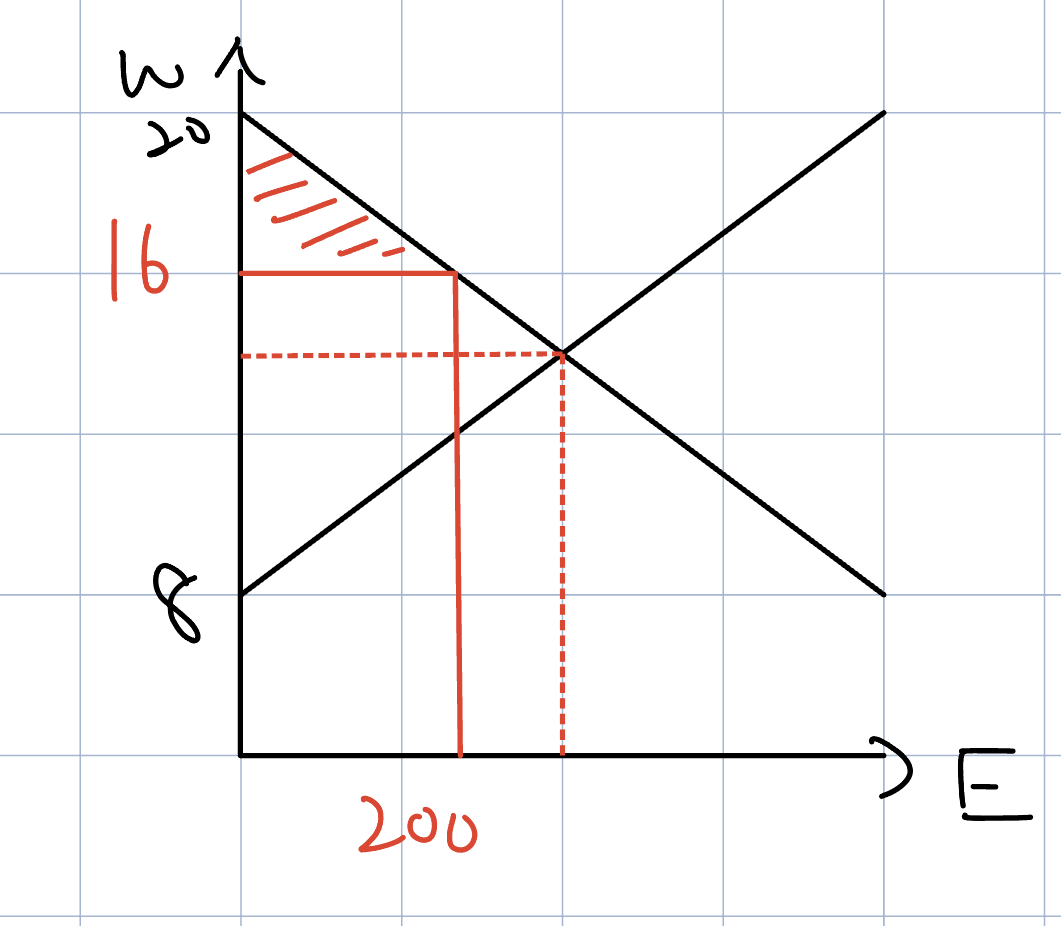
\includegraphics[width=0.5\linewidth]{IMG_82081927AD66-1.jpeg}

    \newpage
    \item [\textbf{Q3}]

    Demand: W = 24 - 0.1E

    If Immigrants Not Allow $\Rightarrow E = 120
    \Rightarrow w = 24 - 0.1(120) = 24 - 12 = 12$

    If Allow $\Rightarrow E = 120 + 20 = 140 \Rightarrow w = 24 - 0.1(140) = 24 - 14 = 10$

    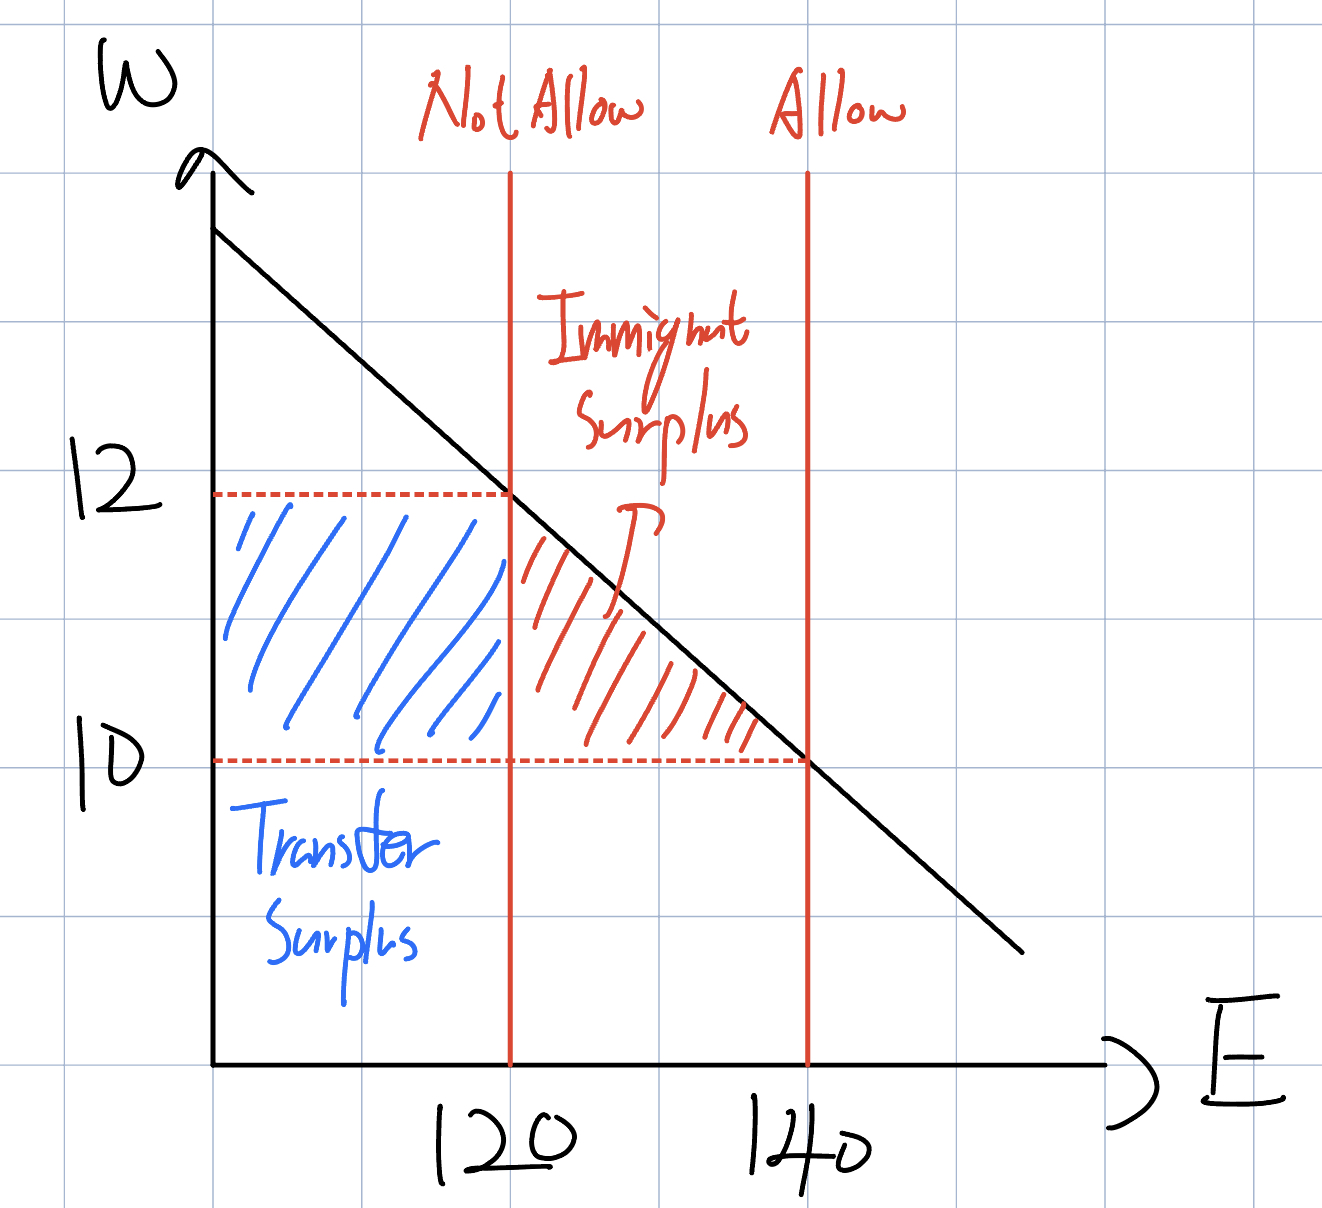
\includegraphics[width=0.5\linewidth]{IMG_848161A42900-1.jpeg}

    Immigrant Surplus = $2 \times \frac{20}{2} = 20$\\
    Transfer Surplus = $2 \times 120 = 240$

    \textbf{Ans}: \\Wage when immigrant are not allow = 12\\ Wage when immigrant are allow = 10\\ Immigrant Surplus = 20 \\ Transferred Surplus = 240
\end{enumerate}

\section{Chapter 6}
\begin{enumerate}
    \item [\textbf{Q1}]

    Plan 1:
    Lifetime income = $100000 + \frac{110000}{1.2} + \frac{90000}{(1.2)^2} = 100000 + 91666.67 + 62500 = 254166.67$
    
    Plan 2:
    Lifetime income = $(-50000) + \frac{180000}{1.2} + \frac{180000}{(1.2)^2} = (-50000) + 150000 + 125000 = 225000$

    Plan 3:
    Lifetime income = $(-50000) + \frac{0}{1.2} + \frac{400000}{(1.2)^2} = (-50000) + 0 + 277777.78 = 227777.78$

    \textbf{Ans}:
    Since Plan 1 generates the largest lifetime income, choosing Plan 1 maximizes Peter’s net present value of his lifetime earnings.

    \newpage
    \item [\textbf{Q2}]

    MRR of Schooling for Carl

    From years 9 to 10 = $\frac{20350 - 18500}{18500} = $ 0.1 = 10\%
    
    From years 10 to 11 = $\frac{22000 - 20350}{20350} =  0.0811 \fallingdotseq 8.1\%$

    From years 11 to 12 = $\frac{23100 - 22000}{22000} = $ 0.05 = 5\%

    From years 12 to 13 = $\frac{23900 - 23100}{23100} =  0.0346 \risingdotseq 3.5\%$

    From years 13 to 14 = $\frac{24000 - 23900}{23900} = $ 0.0042 = 0.42\%

    \textbf{Ans}: 
    
    When the discount rate is 4\% $\Rightarrow$ Quit schooling when years 12

    When the discount rate is 9\% $\Rightarrow$ Quit schooling when years 10
    
    \item [\textbf{Q3}]

    For low ability students $\Rightarrow k - 20000 < 25000 \Rightarrow 25000 + 20000 > k \Rightarrow 45000 > k$

    For high ability students $\Rightarrow k - 8000 > 25000 \Rightarrow 25000 + 8000 < k \Rightarrow 33000 < k$

    \textbf{Ans}:
    $\Rightarrow 33000 < k < 45000$
\end{enumerate}

\end{document}